% \documentclass{article}
\documentclass[fleqn]{article}
\usepackage{import}
\subimport*{../assignment-2/}{macro}

\setlength\parindent{20px}
\setlength{\mathindent}{20pt}

\begin{document}
\title{Homework \#2}
\author{Aaron Chen / aaronyc}
\date{}
\maketitle

% ------ setting ------

\subsection*{A1. Conceptual Questions}

\begin{enumerate}[label=(\alph*)]
\item
Not necessarily. Although number of bathrooms has a large positive weight, removing it and refitting may let other correlated features, such as house size or number of bedrooms, capture similar information. Also, if this feature was causing the model to overfit unusual examples, such as houses with an extreme number of bathrooms, removing it could even decrease test error.

\item
Compared with L2, L1 continues to penalize small nonzero weights strongly near zero, while the L2 penalty becomes very small as weights approach zero; therefore L1 is more likely to push weak feature weights exactly to zero.

\item
Upside: This regularizer can encourage even stronger sparsity, so it may remove weak or noisy features from the model.

Downside: Since the power is less than 1, the regularizer is nonconvex, which can make optimization harder and less reliable.

\item
True. If the step size is too large, gradient descent can overshoot the minimizer and move farther away instead of closer. In that case, the iterates may oscillate or diverge, so the algorithm may not converge.

\item
SGD tries to minimize the difference between the model prediction and the real data by repeatedly updating the model weights. Although each update only uses a small random part of the data, that small part gives a noisy estimate of the full gradient, so over many updates the model usually moves toward lower loss.

\item
Advantage: SGD is cheaper per update than GD because it only uses one example or a small minibatch instead of the full dataset.

Disadvantage: SGD has noisier and less stable updates, so the objective may not decrease smoothly and the step size needs to be chosen carefully.
\end{enumerate}

% ---------------------

\subsection*{A2. Convexity and Norms: Norm Proofs}

\begin{enumerate}[label=(\alph*)]
\item
\begin{enumerate}[label=(\roman*)]
\item Non-negativity:
\begin{align*}
f(x) &= \sum_{i=1}^{n}\abs{x_i} \geq 0 \\
f(x) = 0
&\Leftrightarrow \sum_{i=1}^{n}\abs{x_i} = 0 \\
&\Leftrightarrow \abs{x_i} = 0,\quad \forall i \in \{1,\dots,n\} \\
&\Leftrightarrow x_i = 0,\quad \forall i \in \{1,\dots,n\} \\
&\Leftrightarrow x = 0
\end{align*}

\item Absolute scalability:
\begin{align*}
f(ax)
&= \sum_{i=1}^{n}\abs{a x_i} \\
&= \sum_{i=1}^{n}\abs{a}\abs{x_i} \\
&= \abs{a}\sum_{i=1}^{n}\abs{x_i} \\
&= \abs{a}f(x)
\end{align*}

\item Triangle inequality:
\begin{align*}
(\abs{u}+\abs{v})^2-\abs{u+v}^2
&= u^2 + 2\abs{u}\abs{v} + v^2 - (u+v)^2 \\
&= 2\abs{uv} - 2uv \\
&= 2(\abs{uv} - uv) \geq 0
\end{align*}
\[
\Rightarrow \abs{u+v} \leq \abs{u}+\abs{v}
\]
\begin{align*}
f(x+y)
&= \sum_{i=1}^{n}\abs{x_i+y_i} \\
&\leq \sum_{i=1}^{n}(\abs{x_i}+\abs{y_i}) \\
&= \sum_{i=1}^{n}\abs{x_i}+\sum_{i=1}^{n}\abs{y_i} \\
&= f(x)+f(y)
\end{align*}
\end{enumerate}

\item
\[
x = \begin{bmatrix}1 \\ 0\end{bmatrix},
\qquad
y = \begin{bmatrix}0 \\ 1\end{bmatrix}
\]
\begin{align*}
g(x)
&= \round{\abs{1}^{1/2}+\abs{0}^{1/2}}^2 \\
&= 1
\end{align*}
\begin{align*}
g(y)
&= \round{\abs{0}^{1/2}+\abs{1}^{1/2}}^2 \\
&= 1
\end{align*}
\begin{align*}
g(x+y)
&= g\round{\begin{bmatrix}1 \\ 1\end{bmatrix}} \\
&= \round{\abs{1}^{1/2}+\abs{1}^{1/2}}^2 \\
&= (1+1)^2 \\
&= 4
\end{align*}
\[
g(x+y) = 4 > 2 = g(x)+g(y)
\]
\[
\Rightarrow g(x+y) \nleq g(x)+g(y)
\]
\end{enumerate}

% ---------------------

\subsection*{A3. Convex Sets}

\begin{enumerate}[label=(\roman*)]
\item Panel I: Not convex. If we connect points $b$ and $c$, part of the line segment between them is outside the gray region.

\item Panel II: Convex. For any two points in the gray region, the line segment between them stays inside the gray region.

\item Panel III: Not convex. If we connect points $a$ and $d$, part of the line segment between them is outside the gray region.
\end{enumerate}

% ---------------------

\subsection*{A4. Convex Functions}

\begin{enumerate}[label=(\alph*)]
\item Panel I on $[a,c]$: Convex. The function is U-shaped on this interval, so the line segment between any two points on the graph stays above the function.

\item Panel II on $[a,c]$: Not convex. For example, using points $a$ and $b$, part of the function lies above the line segment between them.

\item Panel III on $[a,d]$: Not convex. For example, using points $a$ and $d$, part of the function lies above the line segment between them.

\item Panel III on $[c,d]$: Convex. On this restricted interval, the function is U-shaped and stays below the line segment between any two points on the graph.
\end{enumerate}

% ---------------------

\subsection*{A5. Lasso on Synthetic Data}

\begin{enumerate}[label=(\alph*)]
\item
\begin{center}
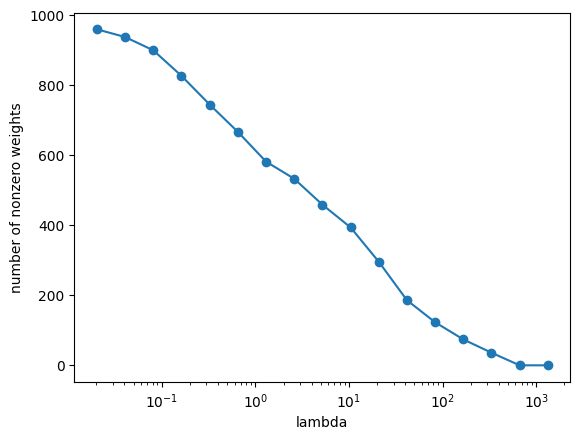
\includegraphics[width=0.8\textwidth]{hw2-A/homeworks/lasso/synthetic_nonzeros_path.png}
\end{center}

\item
\begin{center}
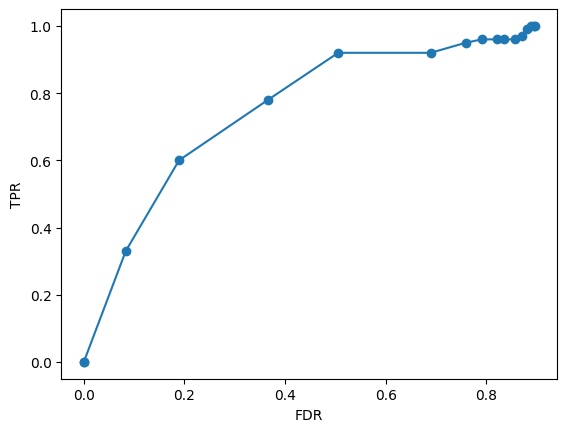
\includegraphics[width=0.8\textwidth]{hw2-A/homeworks/lasso/synthetic_fdr_tpr.png}
\end{center}

\item
As $\lambda$ decreases, the Lasso penalty becomes weaker, so more coefficients become nonzero. This increases the true positive rate by selecting more relevant features, but it also increases the false discovery rate by selecting more irrelevant features.
\end{enumerate}

% ---------------------

\subsection*{A6. Lasso on Crime Data}

\begin{enumerate}[label=(\alph*)]
\item
Three examples are:
\begin{itemize}
\item \texttt{PctHousOwnOcc}: This can vary because of historical housing policies such as zoning, mortgage access, and redlining.
\item \texttt{PctNotHSGrad}: This can vary because of education policies such as school funding, district boundaries, and access to public education.
\item \texttt{pctUrban}: This can vary because of land-use policy, zoning, highway construction, and urban development decisions.
\end{itemize}

\item
Three examples are:
\begin{itemize}
\item \texttt{NumInShelters}: This could be interpreted as a reason for higher crime, but it may instead be a result of poverty, displacement, or lack of housing resources in the community.
\item \texttt{PctVacantBoarded}: This could be interpreted as a reason for higher crime, but boarded vacant housing may also be a result of disinvestment, people moving away, or previous crime in the area.
\item \texttt{LemasPctOfficDrugUn}: This could be interpreted as a reason for higher crime, but police assignment to drug units may be a response to reported crime or enforcement priorities rather than a cause.
\end{itemize}

\item
\begin{center}
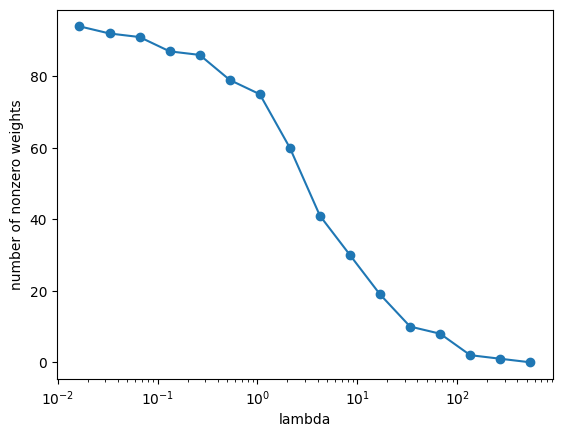
\includegraphics[width=0.8\textwidth]{hw2-A/homeworks/lasso/crime_nonzeros_path.png}
\end{center}

\item
\begin{center}
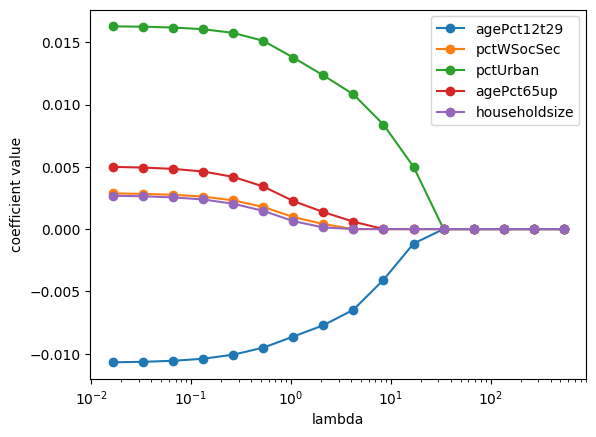
\includegraphics[width=0.8\textwidth]{hw2-A/homeworks/lasso/crime_regularization_paths.png}
\end{center}

\item
\begin{center}
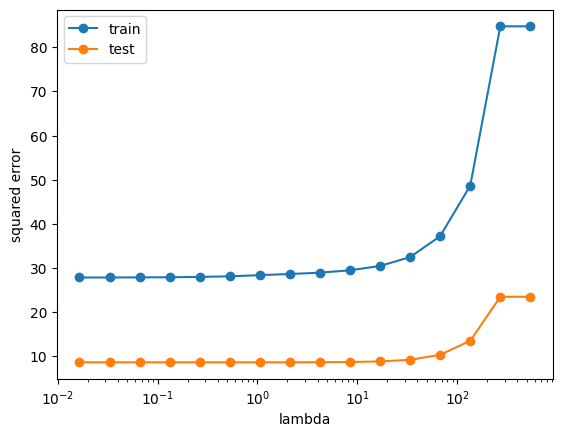
\includegraphics[width=0.8\textwidth]{hw2-A/homeworks/lasso/crime_squared_error.png}
\end{center}

\item
\begin{itemize}
\item Largest positive coefficient: \texttt{PctIlleg}, with coefficient approximately $0.0680$.
\item Most negative coefficient: \texttt{PctKids2Par}, with coefficient approximately $-0.0454$.
\item These coefficients should be interpreted as associations in the fitted model, not causal effects. The positive coefficient means the model predicts higher violent crime rate as \texttt{PctIlleg} increases, while the negative coefficient means the model predicts lower violent crime rate as \texttt{PctKids2Par} increases, holding the other model terms fixed.
\end{itemize}

\item
The politician is confusing correlation with causation. A negative coefficient on \texttt{agePct65up} only shows an association in this observational dataset; it does not imply that moving people over age 65 into high-crime areas would cause crime to decrease.
\end{enumerate}

% ---------------------

\subsection*{A7. Binary Logistic Regression}

\begin{enumerate}[label=(\alph*)]
\item
Let
\[
z_i = y_i(b+x_i^\top w),
\qquad
\mu_i(w,b) = \frac{1}{1+\exp(-z_i)}
\]
\begin{align*}
\frac{\exp(-z_i)}{1+\exp(-z_i)}
&= 1 - \frac{1}{1+\exp(-z_i)} \\
&= 1-\mu_i(w,b)
\end{align*}
\begin{align*}
\nabla_w J(w,b)
&= \frac{1}{n}\sum_{i=1}^{n}
\nabla_w \log(1+\exp(-z_i)) + 2\lambda w \\
&= \frac{1}{n}\sum_{i=1}^{n}
\frac{\exp(-z_i)}{1+\exp(-z_i)}(-\nabla_w z_i) + 2\lambda w \\
&= \frac{1}{n}\sum_{i=1}^{n}
(1-\mu_i(w,b))(-y_i x_i) + 2\lambda w \\
&= \frac{1}{n}\sum_{i=1}^{n}
(\mu_i(w,b)-1)y_i x_i + 2\lambda w
\end{align*}
\begin{align*}
\nabla_b J(w,b)
&= \frac{1}{n}\sum_{i=1}^{n}
\nabla_b \log(1+\exp(-z_i)) \\
&= \frac{1}{n}\sum_{i=1}^{n}
\frac{\exp(-z_i)}{1+\exp(-z_i)}(-\nabla_b z_i) \\
&= \frac{1}{n}\sum_{i=1}^{n}
(1-\mu_i(w,b))(-y_i) \\
&= \frac{1}{n}\sum_{i=1}^{n}
(\mu_i(w,b)-1)y_i
\end{align*}
\begin{align*}
\nabla_w J(w,b)
&= \frac{1}{n}\sum_{i=1}^{n}(\mu_i(w,b)-1)y_i x_i + 2\lambda w \\
\nabla_b J(w,b)
&= \frac{1}{n}\sum_{i=1}^{n}(\mu_i(w,b)-1)y_i
\end{align*}

\item
\begin{enumerate}[label=(\roman*)]
\item Objective plot:
\begin{center}
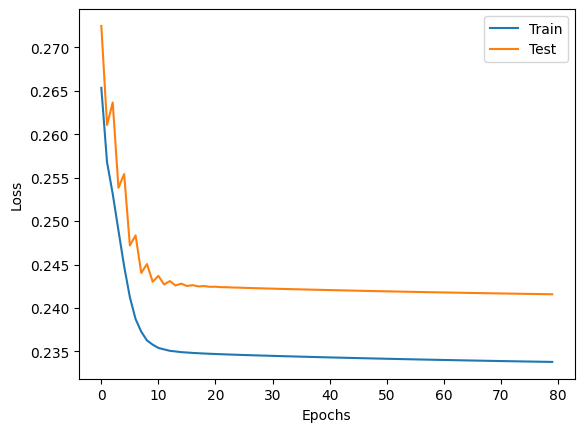
\includegraphics[width=0.8\textwidth]{hw2-A/homeworks/log_regression/gd_objective.png}
\end{center}

\item Misclassification plot:
\begin{center}
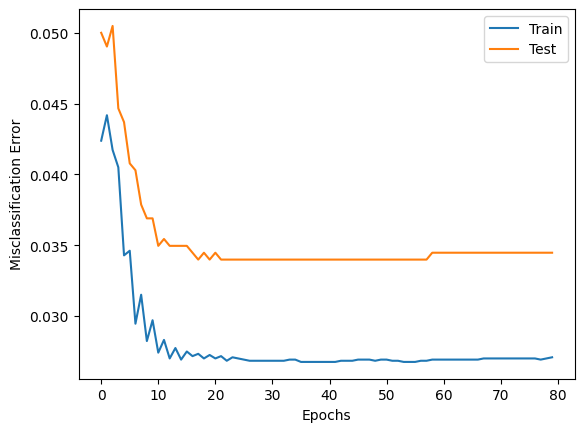
\includegraphics[width=0.8\textwidth]{hw2-A/homeworks/log_regression/gd_misclassification.png}
\end{center}
\end{enumerate}

\item
\begin{center}
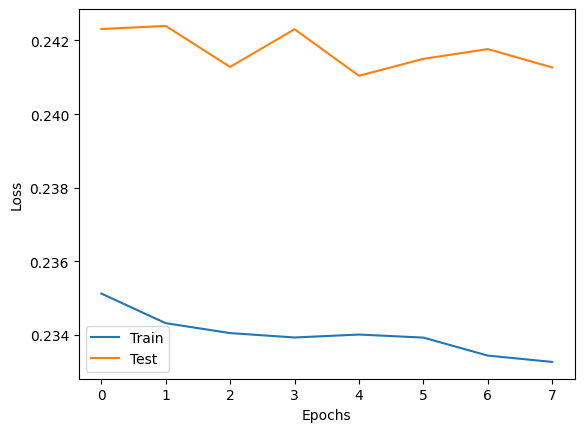
\includegraphics[width=0.8\textwidth]{hw2-A/homeworks/log_regression/sgd1_objective.png}

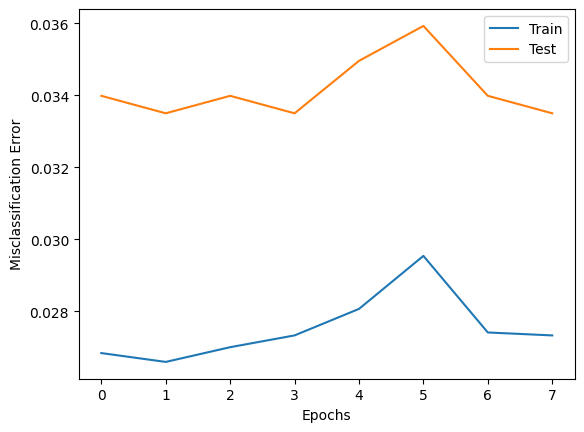
\includegraphics[width=0.8\textwidth]{hw2-A/homeworks/log_regression/sgd1_misclassification.png}
\end{center}

\item
\begin{center}
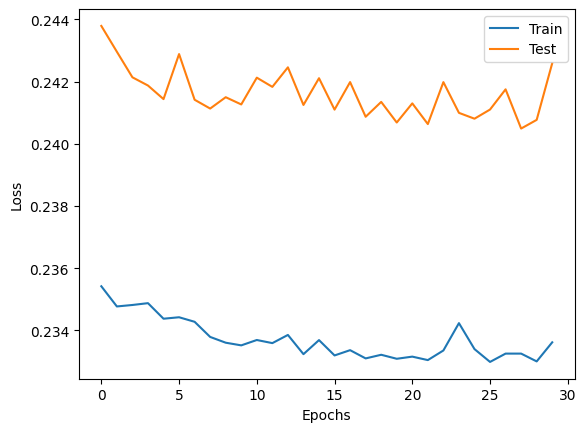
\includegraphics[width=0.8\textwidth]{hw2-A/homeworks/log_regression/sgd100_objective.png}

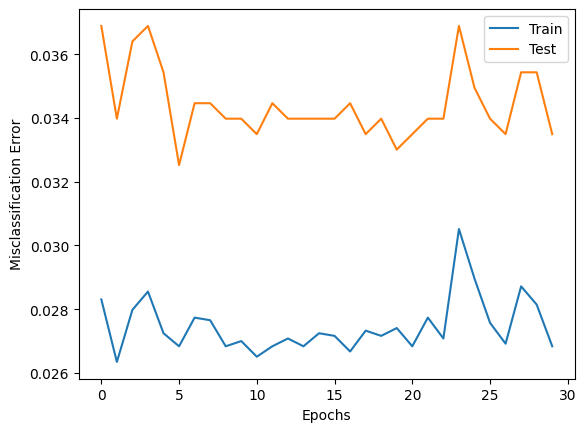
\includegraphics[width=0.8\textwidth]{hw2-A/homeworks/log_regression/sgd100_misclassification.png}
\end{center}
\end{enumerate}

% ---------------------

% Reminder: Because AI help was used, include the required transcript with the submission.

% ------ setting ------

\end{document}
